\documentclass{beamer}




\usepackage[T1,T2A]{fontenc}
\usepackage[utf8]{inputenc}

\usepackage{graphicx}
\usepackage{blindtext}
\usepackage{ mathrsfs }
\usepackage[russian,english]{babel}
%\usepackage{ dsfont }

\author{Деркач Максим Юрьевич}
\title{Криптографические протоколы}
\subtitle{Лекция 7 \\ Протоколы распределения ключей (Часть 1)}


%\usetheme{lucid}
\begin{document}
	\frame {
		\titlepage
	}
	\frame {
		\frametitle{Ссылки}
		
		\begin{enumerate}
			\item ISO/IEC 11770-1:2010 – Information technology – Security techniques – Key management – Part 1: Framework 
			\item ISO/IEC 11770-2:2008 – Information technology – Security techniques – Key management – Part 2: Mechanisms using symmetric techniques 
			\item ISO/IEC 11770-3:2008 – Information technology – Security techniques – Key management – Part 3: Mechanisms using asymmetric techniques 
			\item ISO/IEC 11770-4:2006 – Information technology – Security techniques – Key management – Part 4: Mechanisms based on weak secrets
			
			\item СТБ 34.101.45-2013 "Информационные технологии и безопасность. Алгоритмы электронной цифровой подписи и транспорта ключа на основе эллиптических кривых". \hyperlink{name}{http://apmi.bsu.by/assets/files/std/bign-spec19.pdf} 
			
			\item СТБ 34.101.60-2014 "Информационные технологии и безопасность. Алгоритмы разделения секрета". \hyperlink{name}{http://apmi.bsu.by/assets/files/std/bels-spec12.pdf} 
		\end{enumerate}
	}
	
	\frame{
		\frametitle{Протоколы распределения ключей}
		\framesubtitle{Определения и понятия}
		\textbf{Определение 1}
		
		Протокол распределения ключей (key establishment protocol)- это криптографический протокол, в процессе выполнения которого общий секрет доступен двум или более сторонам для последующего использования в криптографических целях.
		\bigskip
		
		Протоколы распределения ключей подразделяются на два класса:
		\begin{itemize}
			\item протоколы транспортировки ключей,
			\item протоколы обмена ключами.
		\end{itemize}
		
		\bigskip
		
		\textbf{Определение 2}
		
		Протокол транспортировки ключей (key transport)- это протокол, распределения ключей, в котрых один участник создает или другим образом приобретает секрет и безопасным образом передает его другим участникам.
			
	}


	\frame{
		\frametitle{Протоколы распределения ключей}
		\framesubtitle{Определения и понятия}
				
		\textbf{Определение 3}
		
		Протокол обмена ключами (key exchange) - это протокол, распределения ключей, в котрых общий секрет вырабатывается двумя или более участниками как функция от информации.	
		
				
		\bigskip
		
		\textbf{Классификация протоколов распределения ключей}
	
		\begin{itemize}
			\item По типу выработки ключей:
			\begin{enumerate}
				\item обновление ключей (key update) - выработка совершенно нового  ключа, не зависищего от ключей выработанных в прошлых сеансах выполнения ппротокола;
				
				\item выработка производных ключей (key derivation) - вырабока нового ключа на основе уже существующих у участников криптосистемы.
			\end{enumerate}	
		\end{itemize}
		
		}

\frame{
	\frametitle{Протоколы распределения ключей}
	\framesubtitle{Определения и понятия}
	\textbf{Классификация протоколов распределения ключей}
	
	\begin{itemize}
		\item По типу :
		\begin{enumerate}
			\item протоколы с предраспределенными ключами (key pre-distribution) -  протоколы распределения, в которых результирующие ключи полностью определены  априори начальным ключевым материалом (схемы разделения секрета);
			\item протоколы динамического распределения ключей (dynamic key establishment) - протоколы распределения, в которых ключи, вырабатываемые участниками, различны в различных сеансах протокола.
		\end{enumerate}
		
		\item По типу используемых криптосистем:
		\begin{enumerate}
			\item  симметричные;
			\item  асиметричные.
		\end{enumerate}
		
		\item По количеству сторон:
		\begin{enumerate}
			\item  с участием "третьей стороны" (сервер аутентификации, центр распределения ключей, удостоверяющий центр и др.);
			\item  без участия "третьей стороны".
		\end{enumerate}
		
	\end{itemize}
	
	}

\frame{
	\frametitle{Протоколы распределения ключей}
	\framesubtitle{Классификация протоколов распределения ключей}
	
	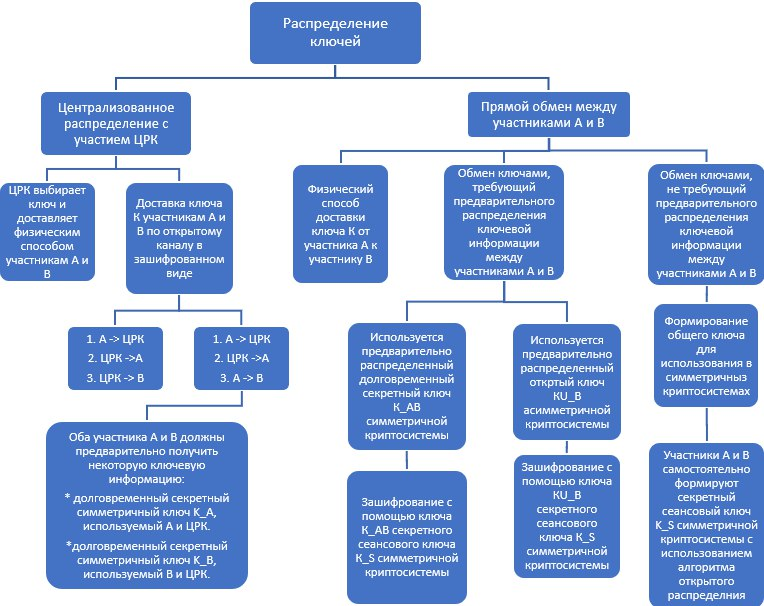
\includegraphics[width=0.9\linewidth]{scheme1.jpg}
}

\frame{
	\frametitle{Протоколы распределения ключей}
	\framesubtitle{Классификация протоколов распределения ключей}
	
	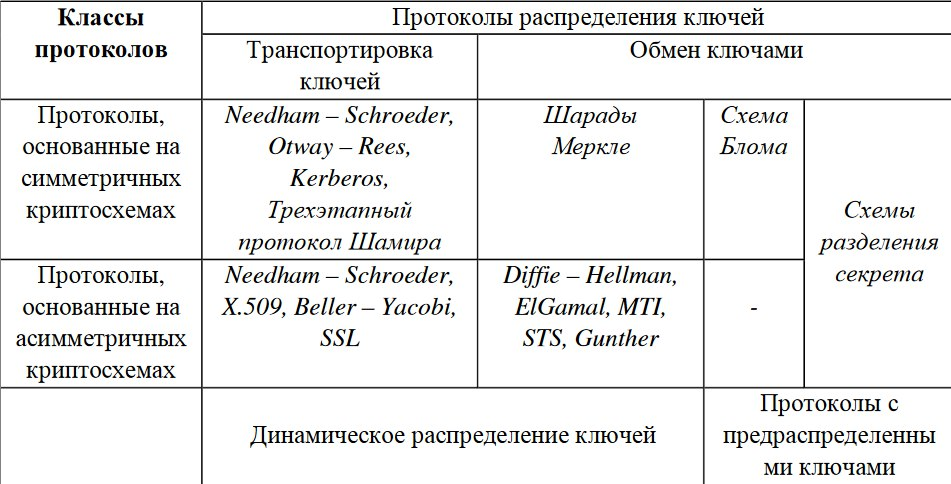
\includegraphics[width=1\linewidth]{scheme2.jpeg}
}

	\frame{
		\frametitle{Протоколы распределения ключей}
		\framesubtitle{ISO/IEC 11770-2}
		
		\textbf{Mech. \#2 (Однораундовый протокол)}
		\begin{enumerate}
			\item $A -> B: E_{K_{AB}}(KS)$
		\end{enumerate}	
		$A$ генерирует $KS$.
		
		\bigskip
		
		\textbf{Mech. \#1 (Однораундовый протокол)}
		
		$TVP$ - переменная
		\begin{enumerate}
			\item $A -> B: TVP$ \\
			$KS = f(K_{AB}, TVP)$ , где $f$ - одностороняя функция.
		\end{enumerate}		
	
		\bigskip
		
		\textbf{Mech. \#3 (Однораундовый протокол)}
		\begin{enumerate}
			\item $A -> B: E_{K_{AB}}(KS || T_A / N_A || ID_B)$
		\end{enumerate}	
		$T_A / N_A$ - проверяет корректность момента времени или номера сессии.\\
		$ID_B$ - против атаки отражения.
	}

		\frame{
		\frametitle{Протоколы распределения ключей}
		\framesubtitle{ISO/IEC 11770-2}
		
		\textbf{Mech. \#4 (Двухраундовый протокол)}
		\begin{enumerate}
			\item $B -> A: R_B$
			\item $A -> B: E_{K_{AB}}(KS || R_B || ID_B)$
		\end{enumerate}	
		
		\bigskip
		
		\textbf{Mech. \#4 (Модификация для двустороней аунтетификации) }
		\begin{enumerate}
			\item $B -> A: R_B$
			\item $A -> B: E_{K_{AB}}(KS || R_A || R_B || ID_B)$
			\item $B -> A: E_{KS}(R_A)$
		\end{enumerate}	
		
		\bigskip
		
		\textbf{Mech. \#6}
	
		$K_A$ - часть ключа $KS$, которая принадлежит $A$.\\
		$K_B$ -	часть ключа $KS$, которая принадлежит $B$.\\
		$KS = f(K_A, K_B)$
		\begin{enumerate}
			\item $B -> A: R_B$
			\item $A -> B: E_{K_{AB}}(K_A || R_A || R_B || ID_B)$
			\item $B -> A: E_{K_{AB}}(K_B || R_A || R_B )$
		\end{enumerate}	

	}


	\frame{
		\frametitle{Протоколы распределения ключей}
		\framesubtitle{ISO/IEC 11770-2}
		
		\textbf{Mech. \#5}
		
		\begin{enumerate}
			\item $A -> B: E_{K_{AB}}(K_A || T_A / N_A || ID_B)$
			\item $B -> A: E_{K_{AB}}(K_B || T_B / N_B || ID_A)$
		\end{enumerate}	
		
	}

	\frame{
		\frametitle{Протоколы распределения ключей}
		\framesubtitle{Бесключевой протокол Шамира (Трёхпроходный протокол Шамира)}
		
		\textbf{Коммутирующее шифрующее преобразование}
		$\forall M, \ K_1,\ K_2 \ : \ E_{K_1}(E_{K_2}(M)) = E_{K_2}(E_{K_1}(M)) $\\
		
		$E_K(M) = M \oplus K$  - слабое преобразование.\\
		$E_{K_A}(M) = M ^ a  mod p$, где $a$ - зависит от $K_A$, $p$ - простое.\\
		
		
		\begin{enumerate}
			\item $A -> B: E_{K_A}(KS)$
			\item $B -> A: E_{K_B}(E_{K_A}(KS))$
			\item $A -> B: D_{K_A}(E_{K_B}(E_{K_A}(KS))) = E_{K_B}(KS)$ 
		\end{enumerate}	
		Отсутствует аутентификация, вместо $B$ злоумышленник может вступить в протокол со своим ключом.
		
	}

	\frame{
		\frametitle{Протоколы распределения ключей}
		\framesubtitle{Трёхсторонние протоколы}
		
		\textbf{Wide-Mouth-Frag}
		\begin{enumerate}
			\item $A -> S: ID_A || E_{K_{AS}}(T_A || ID_B || KS)$
			\item $S -> B: E_{K_{BS}}(T_S || ID_A || KS)$
		\end{enumerate}
		Интервалы времени должны быть достаточно короткими.
		
		\bigskip
		\textbf{Yahalom}
		\begin{enumerate}
			\item $A -> B: ID_A || R_A$
			\item $B -> S: ID_B || E_{K_{BS}}(ID_A || R_A || R_B)$
			\item $S -> A: $\\
		\quad \quad \quad  \quad $ m_a = E_{K_{AS}}(ID_B || KS || R_A || R_B) ||$ \\
		 \quad \quad \quad  \quad $ m_b = E_{K_{BS}}(ID_A || KS)$
			\item $A -> B: m_b || E_{KS}(R_B)$			   
		\end{enumerate}
			
	}

	\frame{
		\frametitle{Протоколы распределения ключей}
		\framesubtitle{Трёхсторонние протоколы}
		
		\textbf{BAN-Yahalom}
		\begin{enumerate}
			\item $A -> B: ID_A || R_A$
			\item $B -> S: ID_B || R_B || E_{K_{BS}}(ID_A || R_A)$
			\item $S -> A: R_B || $\\
			\quad \quad \quad  \quad $m_a = E_{K_{AS}}(ID_B || KS || R_A) ||$\\
			\quad \quad \quad  \quad $m_b = E_{K_{BS}}(ID_A || KS || R_B)$
			\item $A -> B: m_b || E_{KS}(R_B)$			   
		\end{enumerate}
	
		\bigskip
		\textbf{Атака чередования сеансов и подмены типов}
		\begin{enumerate}
			\item $I(A) -> B: ID_A || R_A$
			\item $B -> I(S): ID_B || R_B || E_{K_{BS}}(ID_A || R_A)$
			
			\item[1'] $I(A) -> B: ID_A || (R_A || R_B)$
			\item[2'] $B -> I(S): ID_B || R_B' || E_{K_{BS}}(ID_A || (R_A || R_B))$
			
			\item $-----------$
							      
			\item $I(A) -> B: E_{K_{BS}}(ID_A || R_A || R_B) || E_{R_A}(R_B)$			   
		\end{enumerate}
		
	}

	\frame{
		\frametitle{Протоколы распределения ключей}
		\subtitle{Трёхсторонние протоколы}
		
		\textbf{Needham-Schroeder (NSSK)}
		\begin{enumerate}
			\item $A -> S: ID_A || ID_B || R_A$
			\item $S -> A: E_{K_{AS}}(R_A || ID_B || KS || E_{K_{BS}}(KS || ID_A))$
			
			\item $A -> B: E_{K_{BS}}(KS || ID_A)$
			\item $B -> A: E_{KS}(R_B)$
			\item $A -> B: E_{KS}(R_B - 1)$			   
		\end{enumerate}
		
	}

	\frame{
		\frametitle{Протоколы распределения ключей}
		\framesubtitle{Needham-Schroeder (NSSK)}
		
		
		\textbf{Атака} \\
		
		Если ключ $KS$	скомпрометирован, возможна атака на протокол методом повтора сеанса: берутся	сообщения из прошлого сеанса с ключом $KS^{*}$: 
		
		\begin{enumerate}
			\item $A -> S: ID_A || ID_B || R_A$
			\item $S -> A: E_{K_{AS}}(R_A || ID_B || KS || E_{K_{BS}}(KS || ID_A))$
			
			\item $I(A) -> B: E_{K_{BS}}(KS^{*} || ID_A)$
			\item $B -> I(A): E_{KS^{*}}(R_B)$
			\item $I(A) -> B: E_{KS^{*}}(R_B - 1)$			   
		\end{enumerate}
		
	}

	\frame{
		\frametitle{Протоколы распределения ключей}
		\subtitle{Трёхсторонние протоколы}
		
		\textbf{Протокол Деннинг - Сакко}
		\begin{enumerate}
			\item $A -> S: ID_A || ID_B$
			\item $S -> A: E_{K_{AS}}(ID_B || KS || T_S || E_{K_{BS}}(ID_A || KS || T_S))$
			
			\item $A -> B: E_{K_{BS}}(ID_A || KS || T_S)$
			\item $B -> A: E_{KS}(R_B)$
			\item $A -> B: E_{KS}(R_B - 1)$			   
		\end{enumerate}
	
		\bigskip
		
		\begin{enumerate}
			\item $A -> B: ID_A$
			\item $B -> A: E_{K_{BS}}(ID_A || R_B)$
			\item $A -> S: ID_A || ID_B || R_A || E_{K_{BS}}(ID_A || R_B)$
			\item $S -> A: E_{K_{AS}}(R_A || ID_B || KS || E_{K_{BS}}(KS || R_B || ID_A ))$
			
			\item $A -> B: E_{K_{BS}}(KS || R_B || ID_A )$
			\item $B -> A: E_{KS}(R_B^{'})$
			\item $A -> B: E_{KS}(R_B^{'} - 1)$			   
		\end{enumerate}
		
	}

	
		\frame{
		\frametitle{Протоколы распределения ключей}
		\subtitle{Трёхсторонние протоколы}
		
		
		\textbf{Протокол Отвея - Рисса}\\
		$M$ - ID сеанса. \\
		$v$ - бит направленности. 
		\begin{enumerate}
			\item $A -> B: M || ID_A || ID_B || E_{K_{AS}}(vR_A || M || ID_A || ID_B)$
			\item $B -> S: M || ID_A || ID_B || E_{K_{AS}}(vR_A || M || ID_A || ID_B) || E_{K_{BS}}(R_B || M || ID_A || ID_B)$
			
			\item $S -> B: M || E_{K_{AS}}(R_A || KS) || E_{K_{BS}}(R_B || KS)$
			\item $B -> A: M || E_{K_{AS}}(R_A || KS)$			   
		\end{enumerate}
		
	}
	
	\frame{
	\frametitle{Протоколы распределения ключей}
	\subtitle{Трёхсторонние протоколы}
	
	
	
\textbf{Атака 1}\\
	$KS$ - 64 бита, $M$ - 32 бита, $ID_A, ID_B$ - 16 бит. \\ 
	$len(KS) = len(M + ID_A + ID_A)$
	\begin{enumerate}
		\item[1'] $A -> I(B): M || ID_A || ID_B || E_{K_{AS}}(vR_A || M || ID_A || ID_B)$	
		\item[4'] $I(B) -> A: M || E_{K_{AS}}(R_A || M || ID_A || ID_B)$	   
	\end{enumerate}


		\bigskip
	\textbf{Атака 2}
	\begin{enumerate}
		\item $A -> B: M || ID_A || ID_B || E_{K_{AS}}(vR_A || M || ID_A || ID_B)$
		\item $B -> I(S): M || ID_A || ID_B || E_{K_{AS}}(vR_A || M || ID_A || ID_B) || E_{K_{BS}}(R_B || M || ID_A || ID_B)$
		
		\item $I(S) -> B: M || E_{K_{AS}}(vR_A || M || ID_A || ID_B) || E_{K_{BS}}(R_B || M || ID_A || ID_B)$
		\item $B -> A: M ||E_{K_{AS}}(vR_A || M || ID_A || ID_B) $			   
	\end{enumerate}
	
	}

	\frame{
		\frametitle{Протоколы распределения ключей}
		\subtitle{ISO/IEC 11770-2}
		
		\textbf{Mech. \#10}
		
		\begin{enumerate}
			\item $A -> S: TVP_A || ID_B$
			\item $S -> A: E_{K_{AS}}(TVP_A || KS || ID_B || text_1) || 
						E_{K_{BS}}(T_S / N_S || KS || ID_A || text_2) || $
			\item $A -> B: E_{K_{BS}}(T_S / N_S || KS || ID_A || text_2) || E_{KS}(T_A/N_A || ID_B || text_3)$
			\item $B - >A: E_{KS}(T_B/N_B || ID_A || text_4)$
		\end{enumerate}	
		
	}
	
	
		
	\frame{
		\frametitle{Протоколы распределения ключей}
		\framesubtitle{Протоколы основанные на ассиметричных криптосистемах}
		
		\textbf{Needham-Schroeder Public Key (NSPK)}
		
		\begin{enumerate}
			\item $A -> S: ID_A || ID_B $
			\item $S -> A: E_{K_{S}^{sec}}(K_B^{pub} || ID_B)$
			
			\item $A -> B: E_{K_{B}^{pub}}(K_A || ID_A)$
			\item $B -> S: ID_B || ID_A$
			\item $S -> B: E_{K_{S}^{sec}}(K_A^{pub} || ID_A)$
			
			\item $B -> A: E_{K_{A}^{pub}}(K_B || K_A)$
			\item $A -> B: E_{K_{B}^{pub}}(K_B)$
			\item $A,B:	\ \ \ \ \ KS = f(K_A, K_B)$   
		\end{enumerate}
		
		$E_{K_{S}^{sec}}()$ - подпись на секретном ключе.\\
		$E_{K_{B}^{pub}}()$ - шифрование на открытом ключе.\\
		$f()$ - общеизвестная однонаправленная функция. 
		
	}
	
	\frame{
		\frametitle{Протоколы распределения ключей}
		\framesubtitle{Протоколы основанные на ассиметричных криптосистемах}
		
		\textbf{NSPK без 3-ей стороны}
		
		\begin{enumerate}
			\item $A -> B: E_{K_{B}^{pub}}(K_A || ID_A)$
			\item $B -> A: E_{K_{A}^{pub}}(K_A || K_B)$
			\item $A -> B: E_{K_{B}^{pub}}(K_B)$
			\item $A,B:	\ \ \ \ \ KS = f(K_A, K_B)$   
		\end{enumerate}
		
	}
	
	\frame{
		\frametitle{Протоколы распределения ключей}
		\framesubtitle{Смешанные протоколы}
		
		\textbf{EKE(Encrypted Key Exchange)}\\
		$K_{AB} = P $ - пароль
		\begin{enumerate}
			\item $A -> B: ID_A || E_P(K_A^{pub})$
			\item $B -> A: E_P(E_{K_A^{pub}}(KS))$
			\item $A -> B: E_{KS}(R_A)$
			\item $B -> A: E_{KS}(R_A || R_B)$	
			\item $A -> B: E_{KS}(R_B)$		   
		\end{enumerate}
		
		\bigskip
		
		\textbf{Bilateral Key Exchange with Public Key}\\
		\begin{enumerate}
			\item $B -> A: ID_B || E_{K_A^{pub}}(R_B || ID_B)$
			\item $A -> B: E_{K_B^{pub}}(h(R_B) || R_A || ID_A || KS)$
			\item $B -> A: E_{KS}(h(R_A))$   
		\end{enumerate}
	}
	
	
	\frame{
		\frametitle{Протоколы распределения ключей}
		\framesubtitle{Протоколы с использованием ЭЦП}
		
		\textbf{Сертификаты открытых ключей}
		$cert_A = (ID_A || K_A^{pub} || t || sign_T(ID_A || K_A^{pub} || t))$
		
		\bigskip	
		
		\textbf{X.509}\\
		$d_A = (T_A || R_A || ID_B || text_1 || E_{K_B^{pub}}(K_A))$ \\
		
		$d_B = (T_B || R_B || ID_A || text_2 || E_{K_A^{pub}}(K_B))$
		\begin{enumerate}
			\item $A -> B: cert_A || d_A || sign_A(d_A)$
			\item $B -> A: cert_B || d_B || sign_B(d_B)$
			
			\item $A -> B: R_B || ID_B || sign_A(R_B || ID_B)$
			\item $A,B:\ \ \ \ \ KS = f(K_A, K_B)$
		\end{enumerate}
		
		Шаг (3) необязателен, выполняется только если нужно подтвержденрие.		
	}
	
	\frame{
		\frametitle{Протоколы распределения ключей}
		\framesubtitle{Протоколы с использованием ЭЦП}
		
		\textbf{Денниг -Сакко}\\
		\begin{enumerate}
			\item $A -> S: ID_A || ID_B$
			\item $S -> A: cert_A || cert_B$
			\item $A -> B: cert_A || cert_B || E_{K_B^{pub}}(KS || t_A || sign_A(kS || T_A))$
			\item $A,B:\ \ \ \ \ KS = f(K_A, K_B)$
		\end{enumerate}
		
		Шаг (3) необязателен, выполняется только если нужно подтвержденрие.		
	}
	
	\frame{
		\frametitle{Протоколы распределения ключей}
		\framesubtitle{}
		
		\textbf{Протокол MTI}
		
		\begin{enumerate}
			\item Предварительный этап: \\
			Выбираются следующие параметры: $p, \alpha$, где $p$ - простое число, $a \in Z^{*}_p$\\
			$A$ выбирает $a,\ 1 \leq a \leq p -2$, $z_A = \alpha ^ a\ (mod\ p)$.\\
			$B$ выбирает $b,\ 1 \leq b \leq p -2$, $z_B = \alpha ^ b\ (mod\ p)$.\\
			\item $A -> B: m_{AB} = \alpha^x\ (mod\ p),\ 1 \leq x \leq p - 2,\ x $ - случайное
			\item $B -> A: m_{BA} = \alpha^y\ (mod\ p),\ 1 \leq y \leq p - 2,\ y $ - случайное
		\end{enumerate}
		
		\bigskip		
		Варианты построения ключа:\\
		\begin{table}[]
			\begin{tabular}{llllll}
				№&  $m_{AB}$&  $m_{BA}$&  $K_A$&  $K_B$&  K\\
				1&  $\alpha^x$&  $\alpha^y$&  $m_{BA}^a z^x_B$&  $m_{AB}^b z^y_A$&  $\alpha^{bx+ay}$\\
				2&  $z^x_B$&  $z^y_A$&  $m_{BA}^{a^{-1}}\alpha^x$&  $m_{AB}^{b^{-1}}\alpha^y$&  $\alpha^{x+y}$\\
				3&  $z^x_B$&  $z^y_A$&  $m_{BA}^{a^{-1}x}$&  $m_{AB}^{b^{-1}y}$&  $\alpha^{xy}$\\
				4&  $z^x_B$&  $z^Y_A$&  $m_{BA}^{x}$&  $m_{AB}^{y}$& $\alpha^{bxay}$
			\end{tabular}
		\end{table}
	}


	\frame {
	\begin{figure}
		
\includegraphics[width=0.8\linewidth]{memes1.jpeg}
		
	\end{figure}
	}

\end{document}